\subsection{Trello}

Pour remplacer les post-it utilisé par la méthode scrum, nous avons cherché plusieurs solution informatisé.
Les première assez complexe proposait tout un environnement adapté à cette méthode, incluant directement tous les test d'intégration continue préconisé par l'extreme programming,
cependant au vus de la difficulté a mettre en place nous nous somme tourné vers une solution n'offrant que la fonctionnalité la plus essentiel, la gestion des user history et du backlog.
Au début nous utilisions des post-it accroché à un mûr, mais nous somme rendu compte que leurs nombres devenais conséquent et qu'il nous était difficile de trouver un endroit pour les stocker qui soit à la fois accessible de tous et ne gênant pas les personnes extérieurs au projet (mobilisation d'une salle pour notre backlog).*
Au final nous nous somme tourné vers une solution web, \textit{Trello}, qui offre une plus grande flexibilité dans la rédaction de contenu d'une user history (annotation, ajout de check list, label ...).

\begin{figure}[h!]
	\centering
	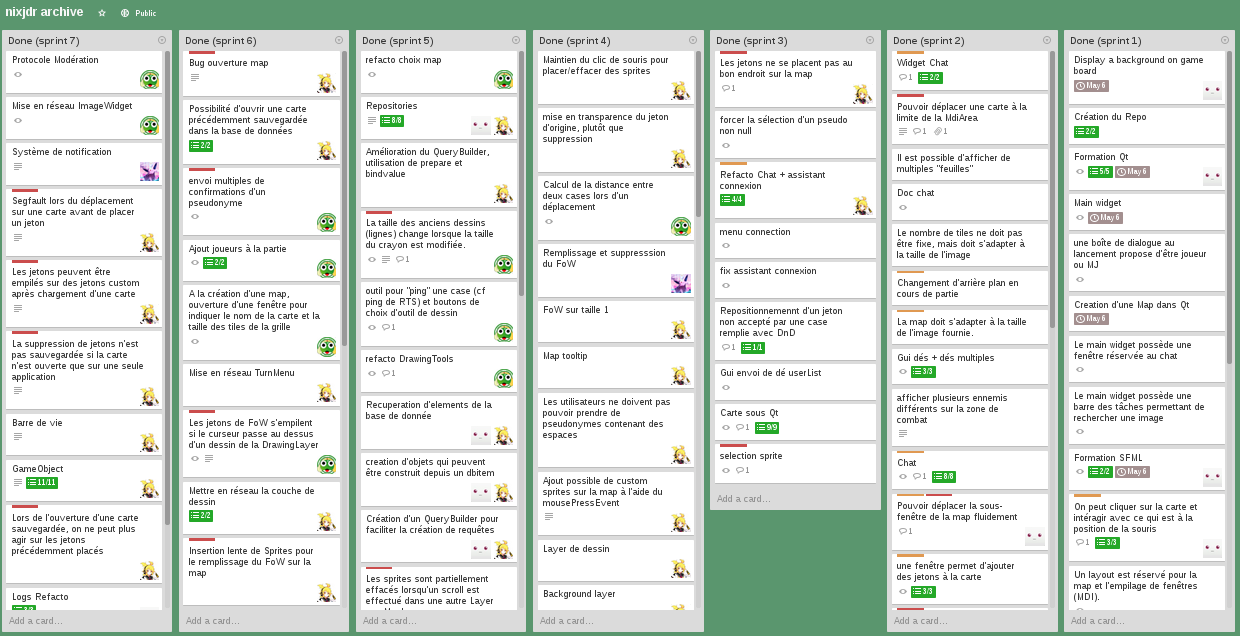
\includegraphics[width=1\textwidth]{img/trello_archive.png}
	\caption{Archive de notre board sur Trello}
\end{figure}
